\chapter{Aktuelle Themen}
\label{chap:aktuelles}

Durch den enormen Anstieg der Containernutzung im Cloud-Umfeld werden zunehmend Probleme ersichtlich, die der in \fref{sec:funktionsweise} beschriebenen Funktionsweise geschuldet sind. Neben der Mitnutzung des Kernels und den damit verbundenen Risiken durch Bugs und sicherheitsrelevante Probleme ist auch die Verwaltung und Organisation der Container-Architekturen zunehmend schwieriger. Neben diesen Problemen entstehen aber auch neue Innovationen rund um Container, z.B. die Serverless-Technologien. Hierbei werden einzelne Module auf Cloud-Plattformen wie Amazon AWS ausgeführt, ohne das Entwickler etwas von Containern und Konfigurationen wissen müssen.

Im folgenden Kapitel sollen aktuelle Probleme erläutert und potentielle Lösungen aufgezeigt werden. Zudem wird am Beispiel der Serverless-Technologie erklärt, wie Container aktuell Anwendung finden.

\section{Security}
\label{sec:aktuellesSecurity}

"Container sind keine Sandbox" \citep{OpenSourcingGVisoraSandboxedContainerRuntime}. Sandboxes sind ein Mechanismus, um laufende Programme zu separieren, damit Schwachstellen in einem Programm keine Auswirkungen auf andere Programme haben. Dies ist bei Containern nur bedingt der Fall. Schwachstellen in einzelnen Prozessen, die innerhalb eines Containers isoliert sind betreffen weitesgehend nur den isolierten Prozess. Sicherheitslücken im Linux-Kernel verbreiten sich allerdings vom Host in jeden Container und werden nicht isoliert.

Ein Beispiel für solch eine Lücke, die genutzt werden konnte, um administrative Rechte innerhalb eines Containers und somit Zugriff auf den übergelegenen Host zu erhalten, ist Dirty COW. Dabei handelte es sich um eine Schwachstelle im Linux-Kernel, die innerhalb der Hauptspeicherverwaltung zu einer Priviledge-Escalation führte \citep{DirtyCOWCVE20165195}. Noch heute sind einige Systeme, die für Container als Host dienen, von dieser Schwachstelle betroffen.

Viele dieser Probleme lassen sich aufgrund der in \fref{sec:funktionsweise} erklärten Funktionsweise von Containern nur schwer umgehen. Durch die größere Nutzung fallen allerdings immer mehr solcher Fehler im Linux-Kernel auf und können behoben werden. Um eine bessere Sicherheit zu gewähren kommen mittlerweile vermehrt die in \fref{sec:compVMbased} beschriebenen VM-basierten Container-Runtimes zum Einsatz.

\section{Orchestrierung}
\label{sec:aktuellesOrchestrierung}

Google setze bereits 2014 stark auf Container. So lief innerhalb Googles Cloud-Platform alles auf Containerbasis und Google startete 2 Milliarden Container jede Woche \citep{ContainersatScale}. Diese massive Zahl an Containern führte zur dringenden Not einer Software, die all diese Container verwaltet, startet, stoppt und überwacht. Dies führte 2014 zum Release der Software Kubernetes, einer Orchestrierungsplattform für containerisierte Anwendungen. \gls{acr-k8} erlaubt es, mittels einer \gls{acr-yml}-Konfiguration, wie in \fref{lst:k8yaml}, ein Cluster an Containern zu spezifizieren, skalieren und bereitzustellen. Dabei verwendet Kubernetes das Konzept Pods, welche die kleinste Einheit bildet. Zu beginn setze \gls{acr-k8} ausschließlich auf Docker Container, mittlerweile wird dies allerdings durch das \gls{acr-cri} vermieden. So können auch rkt, LXD oder beliebige andere Container-Runtimes in Clustern verwendet werden (siehe \fref{fig:k8cri}).

\begin{listing}[hp]
	\begin{minted}[breaklines, breakafter=/]{yaml}

apiVersion: apps/v1 # for versions before 1.9.0 use apps/v1beta2
kind: Deployment
metadata:
    name: nginx-deployment
spec:
    selector:
        matchLabels:
            app: nginx
    replicas: 2 # tells deployment to run 2 pods matching the template
    template: # create pods using pod definition in this template
        metadata:
        # unlike pod-nginx.yaml, the name is not included in the meta data as a unique name is
        # generated from the deployment name
            labels:
                app: nginx
        spec:
            containers:
            - name: nginx
              image: nginx:1.7.9
              ports:
              - containerPort: 80
	\end{minted}
	\caption{Kubernets YAML-Kofiguration für nginx Cluster \citep{KubernetesDocumentation}}
	\label{lst:k8yaml}
\end{listing}

\begin{figure}[h]
	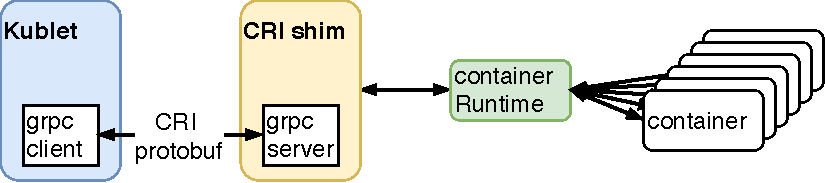
\includegraphics[scale=1]{bilder/cri.pdf}
	\caption{Container Runtime Interface Aufbau \citep{KubernetesDocumentation}}
	\label{fig:k8cri}
\end{figure}

\section{Serverless}
\label{sec:aktuellesServerless}

Ein aktueller Anwendungsfall für Container ist die Serverless-Technologie. Egal ob Amazon Lambdas oder andere \gls{acr-faas} Anbieter, im Hintergrund dieser Technologie stehen immer Container-Pools, die genutzt werden um einzelne minimale, zustandslose Funktionen auszuführen.

\todo{Beschreibung Serveless Funktion, FaaS als Computing Unit, ...}